\documentclass{article}

% if you need to pass options to natbib, use, e.g.:
% \PassOptionsToPackage{numbers, compress}{natbib}
% before loading nips_2018

% ready for submission
% \usepackage{nips_2018}

% to compile a preprint version, e.g., for submission to arXiv, add
% add the [preprint] option:
% \usepackage[preprint]{nips_2018}

% to compile a camera-ready version, add the [final] option, e.g.:
\usepackage[final]{nips_2018}

% to avoid loading the natbib package, add option nonatbib:
% \usepackage[nonatbib]{nips_2018}

\usepackage[utf8]{inputenc} % allow utf-8 input
\usepackage[T1]{fontenc}    % use 8-bit T1 fonts
\usepackage{hyperref}       % hyperlinks
\usepackage{url}            % simple URL typesetting
\usepackage{booktabs}       % professional-quality tables
\usepackage{amsfonts}       % blackboard math symbols
\usepackage{nicefrac}       % compact symbols for 1/2, etc.
\usepackage{microtype}      % microtypography
\usepackage{graphicx}


\title{Music Generation based on Emotions}


\author{
  Sungpyo Cho\\
  Department of Computer Science\\
  Korea University\\
  \texttt{korra0501@gmail.com}
  \and
  \textbf{Taelim Hwang}\\
  Department of Computer Science\\
  Korea University\\
  \texttt{ghkdxofla@gmail.com}
  }
  
  

\begin{document}
% \nipsfinalcopy is no longer used

\maketitle

\begin{abstract}
    Our framework is divided into two models, the text-based sentiment classification model, and the music generation model. The sentiment classification model is implemented with TF-IDF and logistic regression classifier, and the model will classify given text into sentiment categories. After classification, the music would be generated by model which uses Char-based RNN architecture and GAN[1]. Our approach is expected to generate music which reflects emotion and sentiment.
\end{abstract}

\section{Introduction}

Music can be associated with human emotions according to each genre. For example, gloomy music is related to negative emotions, and calm music is related to positive, calm emotions. Human feelings are also contained in sentences. Articles containing emotional words, such as depressed or happy, indicate the author's emotional state. The purpose of this project is to extract the emotional state of the sentence through the sentence analysis, then to generate the music suitable for the emotional state of the sentence. For this purpose, the final goal is to utilize word vectorization, RNN, and GAN, and build optimized models to create natural and appropriate music for people to listen.

\begin{figure}[hbt!]
  \centering
  %\fbox{\rule[-.5cm]{0cm}{4cm} \rule[-.5cm]{4cm}{0cm}}
  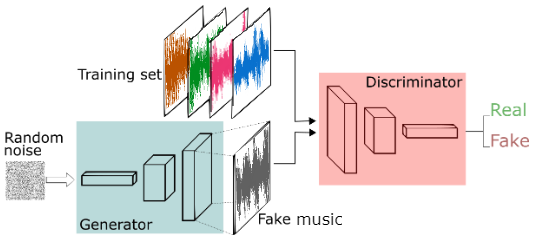
\includegraphics[scale=0.4]{./image/deep_gan.png}
  \caption{basic GAN architecture}
\end{figure}

\section{Differences from previous studies}

In the previous study, melodies were created by learning the melody of music through deep learning or by combining sample bits. On the other hand, research on creating music with different moods based on emotions has not progressed much. There has been studies which tried to extract emotional states by recognizing human expressions and to produce related melodies, but there were some limitations regarding to emotional state definition and outcomes. That is, the extraction of emotions and the creation of appropriate melodies are still a slow study. Our model aims to produce music only with the emotion of the sentence. It could transform literature such as novels and poems which are rich in human emotions, into sounds and produce music that is tailored to individual emotions of people.

\section{Benefits from research}

Our model is expected to easily produce music that fits the text by composing music through the kind of emotions it has. If this technology is later linked to voice recognition, it could provide emotional stability through customized music based on user's emotional state on AI speakers. In addition, it will be possible to reduce the burden of copyright on existing music use and to write music easily without professional knowledge.

\section{Model and Dataset}

First, there are few performance algorithms in emotional analysis that go beyond the TF-IDF and logistic regression models. Therefore, we decided to use this algorithm to classify sentiment from texts. We chose Sentiment140 dataset, which originated from Stanford University. If possible, we will try to analyze emotions through the implementation of Tree-LSTM model[2].

Secondly, based on emotion extracted from emotional analysis, our network will produce music that matches the mood. It uses char-based RNN architecture and plans to increase accuracy even more by using GAN. 



\begin{figure}[hbt!]
  \centering
  %\fbox{\rule[-.5cm]{0cm}{4cm} \rule[-.5cm]{4cm}{0cm}}
  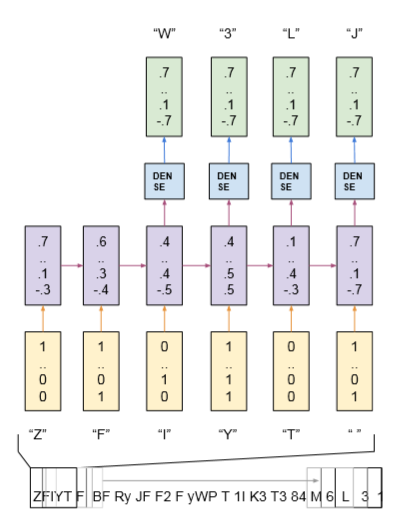
\includegraphics[scale=0.5]{./image/char-based_RNN_arch.png}
  \caption{char-based RNN architecture}
\end{figure}

Music datasets will include Open Datasets, music samples from Musicradar, and private music datasets. Datasets will be grouped by genre and emotion. Model structures and datasets will be defined more specifically as the project progress. proposals and become more specific. We aim to generate music which is pleasant to hear and is appropriate according to the mood of the text.

\section*{References}

\small
[1] Goodfellow, I., Pouget-Abadie, J., Mirza, M., Xu, B., Warde-Farley, D., Ozair, S., ... Bengio, Y. (2014). Generative adversarial nets. In Advances in neural information processing systems (pp. 2672-2680).

[2] Tai, K. S., Socher, R., Manning, C. D. (2015). Improved semantic representations from tree-structured long short-term memory networks. arXiv preprint arXiv:1503.00075.

\end{document}
